\documentclass[a4paper,11pt]{article}
\usepackage{color}
\usepackage{graphicx}
\usepackage{subcaption}
\usepackage{amsmath}
\usepackage{tikz}
\usepackage{listings}
\definecolor{codegreen}{rgb}{0,0.6,0}
\definecolor{codegray}{rgb}{0.5,0.5,0.5}
\definecolor{codepurple}{rgb}{0.58,0,0.82}
\definecolor{backcolour}{rgb}{0.95,0.95,0.92}
 
\lstdefinestyle{mystyle}{
    backgroundcolor=\color{backcolour},   
    commentstyle=\color{codegreen},
    keywordstyle=\color{magenta},
    numberstyle=\tiny\color{codegray},
    stringstyle=\color{codepurple},
    basicstyle=\footnotesize,
    breakatwhitespace=false,         
    breaklines=true,                 
    captionpos=b,                    
    keepspaces=true,                 
    numbers=left,                    
    numbersep=5pt,                  
    showspaces=false,                
    showstringspaces=false,
    showtabs=false,                  
    tabsize=2
}
 
\lstset{style=mystyle}
\usetikzlibrary{automata,positioning}

\graphicspath{ {images/} }
\begin{document}
\title{\color{red}CARNEGIE MELLON UNIVERSITY\\
APPLIED STOCHASTIC PROCESSES  (COURSE 18-751)\\
HOMEWORK 9}
\author{Daniel Marew}
\date{\today}
\clearpage\maketitle

\thispagestyle{empty}
\newpage
I collaborated with :\\
\hspace*{6cm}
Nebyou Yismaw\\
\hspace*{6cm}
Daniel    Nkemelu\\
\hspace*{6cm}
Agatha Niwomugizi
\thispagestyle{empty}
\newpage
\clearpage

\setcounter{page}{1}
\section*{Q.1}
\subsection*{(a)}

\begin{figure}[h]
\centering
 % \hspace*{-2cm}
   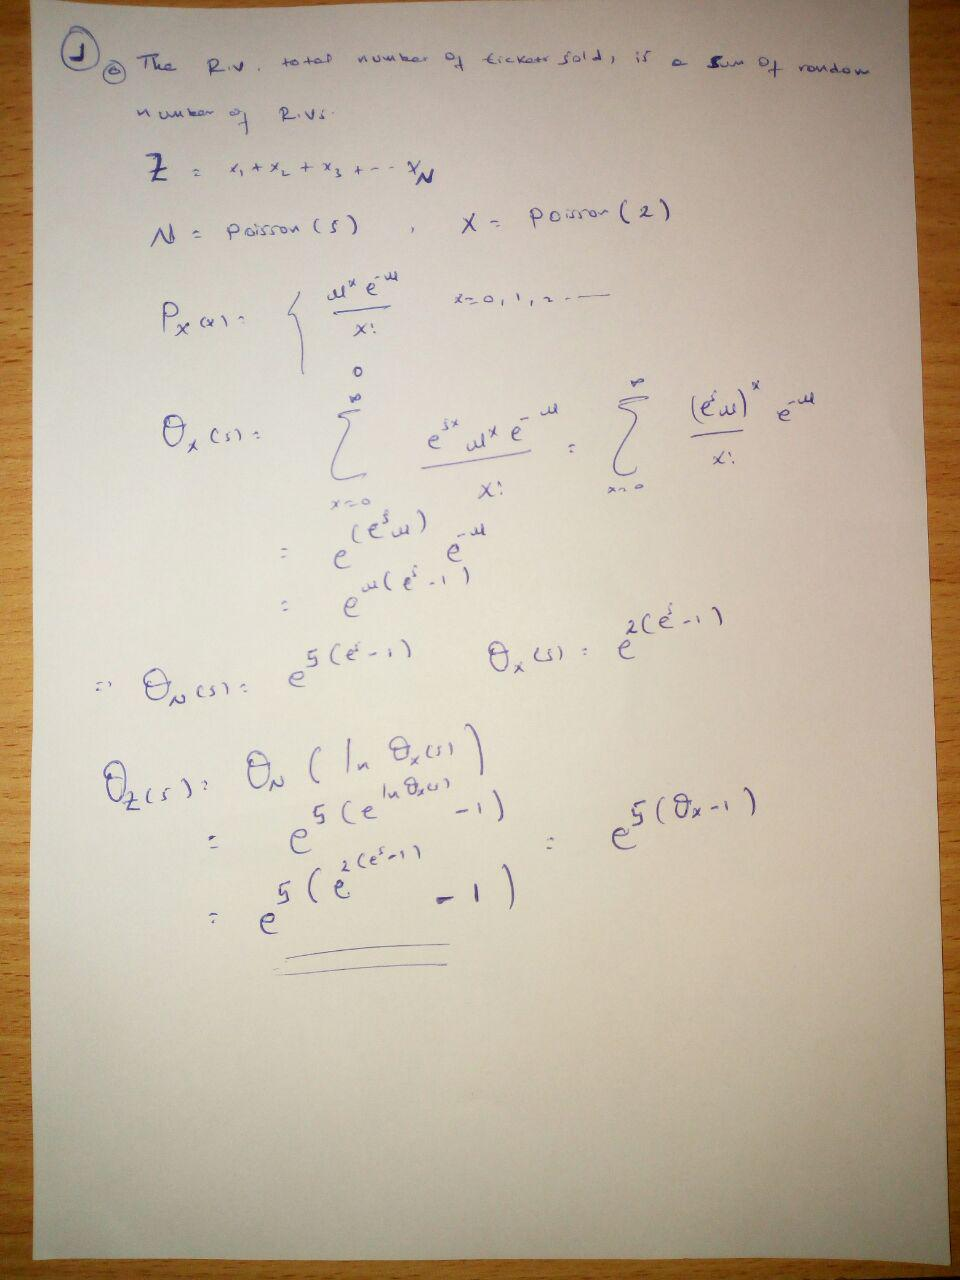
\includegraphics[scale=0.45]{q1_a}
   %\caption{}\label{fig:q3}
\end{figure}
\clearpage
\newpage
\subsection*{(b)}
\begin{figure}[h]
\centering
  %\hspace*{-2cm}
   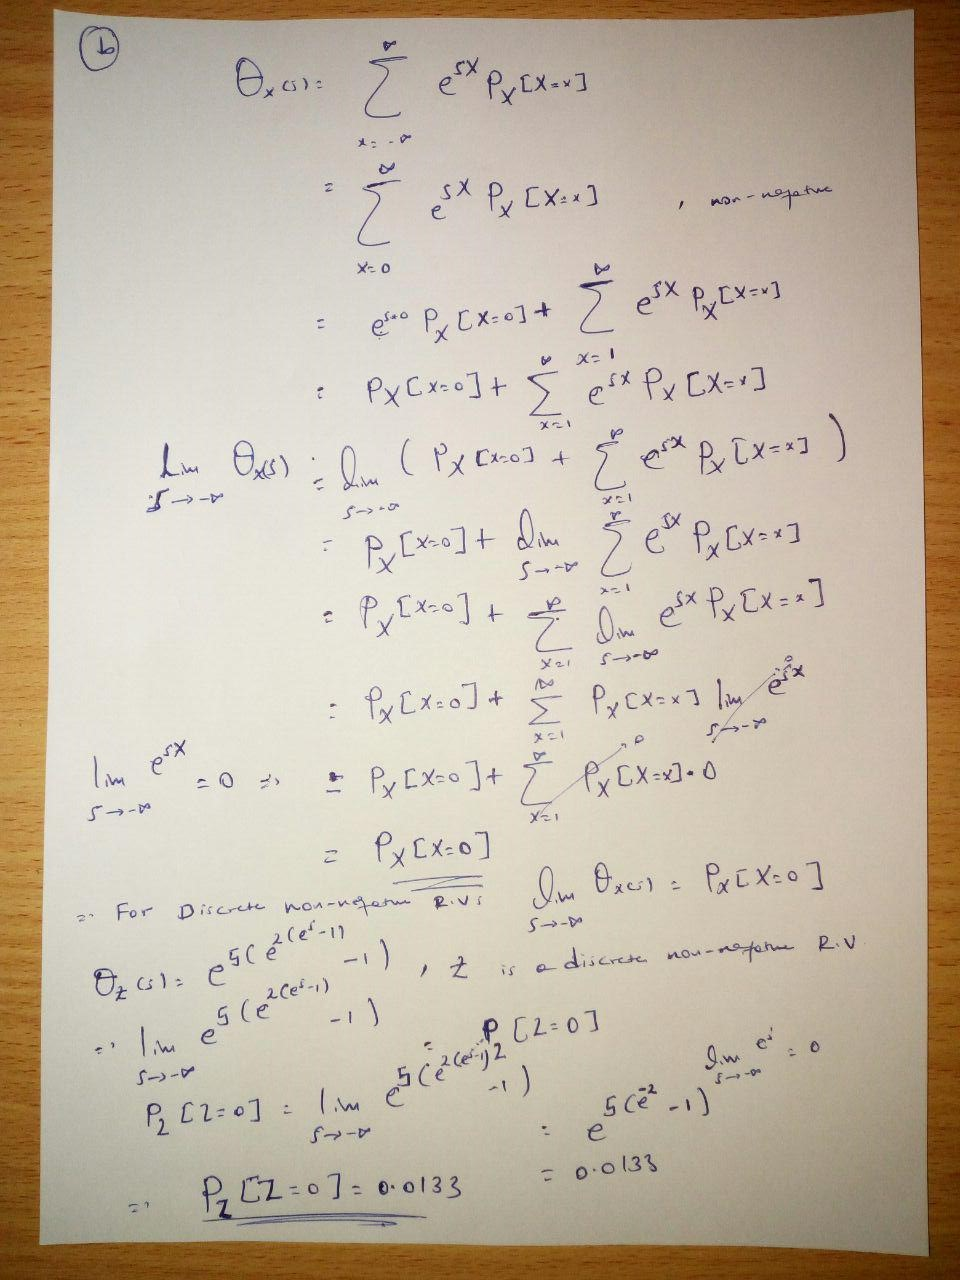
\includegraphics[scale=0.45]{q1_b}
   %\caption{}\label{fig:q3}
\end{figure}
\clearpage
\newpage
\subsection*{(c,d)}
\begin{figure}[h]
  %\hspace*{-2cm}
  \centering
   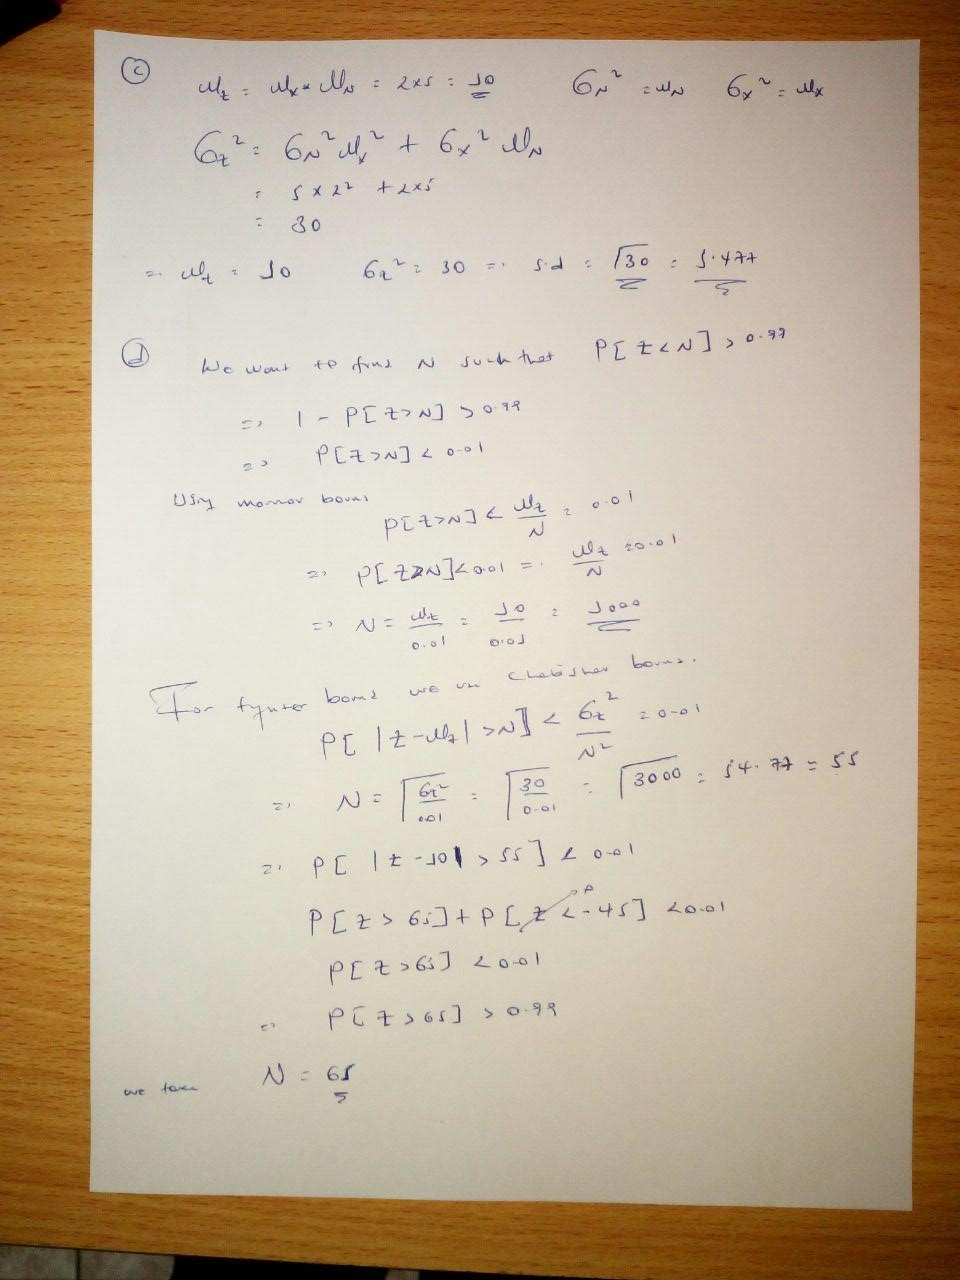
\includegraphics[scale=0.45]{q1_c}
   %\caption{}\label{fig:q3}
\end{figure}
\clearpage
\newpage
\section*{Q.2}
\subsection*{(a,b,c)}
\begin{figure}[h]
  %\hspace*{-2cm}
  \centering
   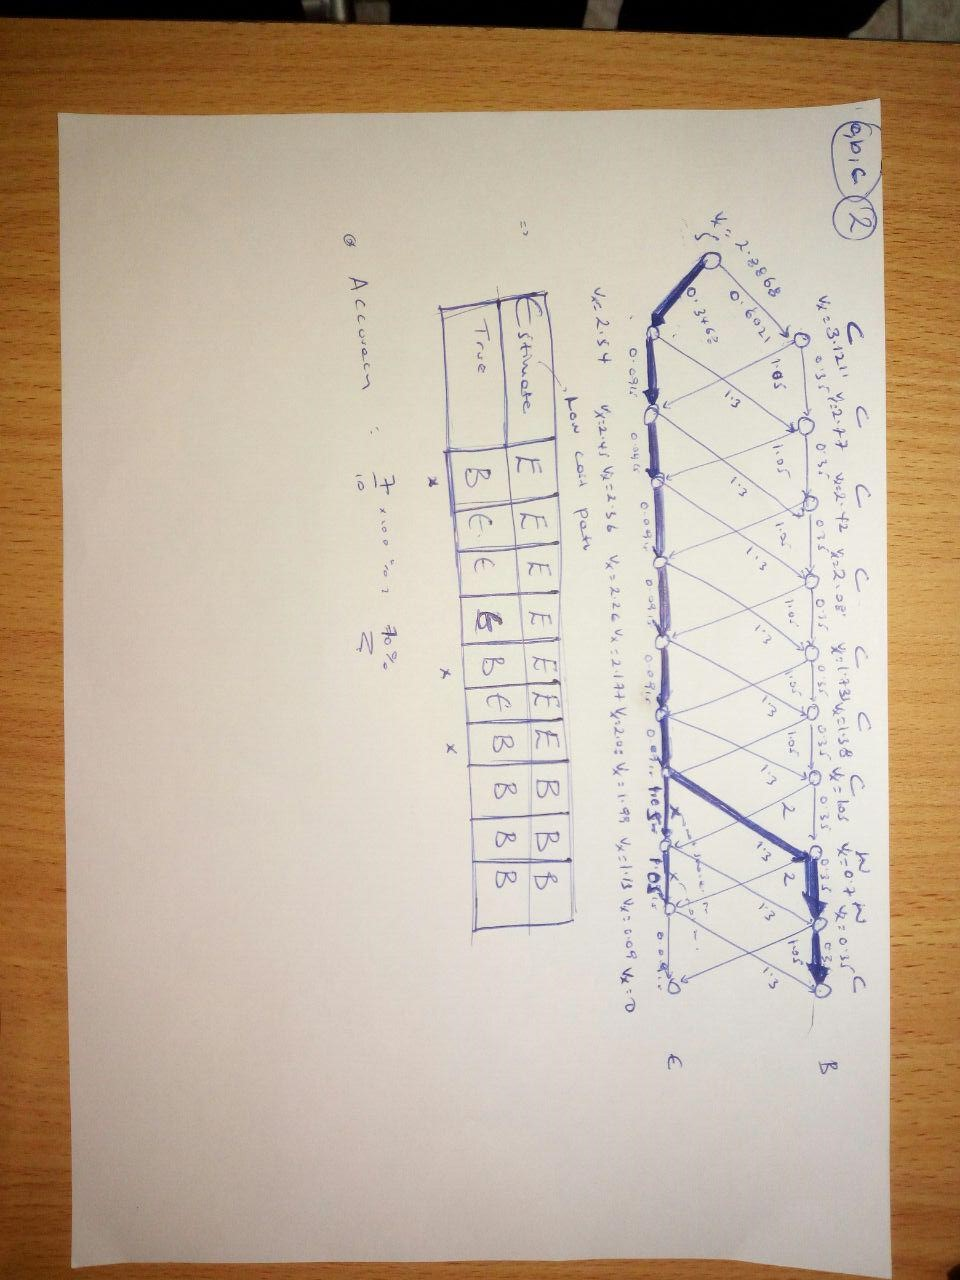
\includegraphics[scale=0.45]{q2_a}
   %\caption{}\label{fig:q3}
\end{figure}
\clearpage
\newpage
\subsection*{(d)}
\begin{figure}[h]
  \hspace*{-5cm}
   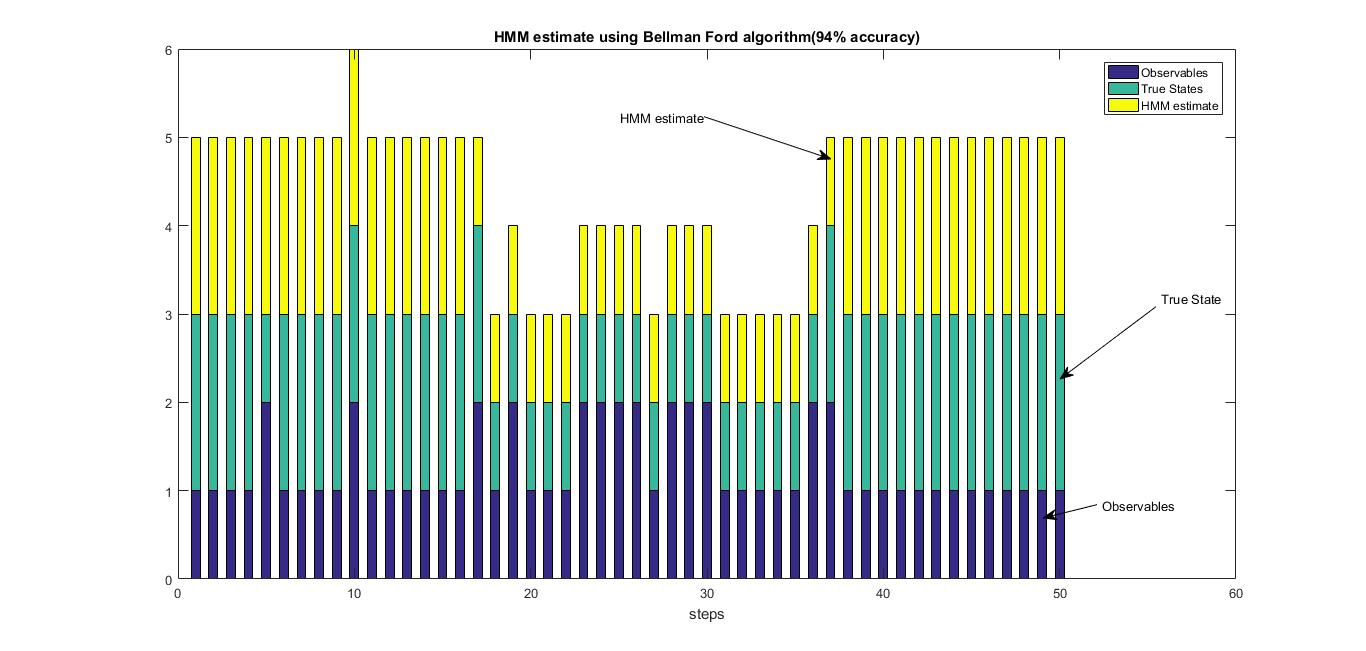
\includegraphics[scale=0.45]{q2_d}
   \caption{HMM with Bellman Ford (94\% accuracy)}\label{fig:q2_d}
\end{figure}
\quad \\
$Accuracy = 94\%$\\
Errors typically occur at transitions\\
\textbf{Interpretation of the graph}\\\\
Observables (length of the bar)\\\\
\quad 1: Correct\\
\quad 2: Wrong\\\\
True states and Estimate(length of the bar)\\\\
\quad 1: Bored\\
\quad 2: Engaged\\\\
To check the accuracy of the estimate, compare the lengths of the estimate and the true value.
\clearpage
\newpage
\section*{Q.3 Kalman Filter}
\subsection*{(a)}

\begin{figure}[h]
  \hspace*{-5cm}
   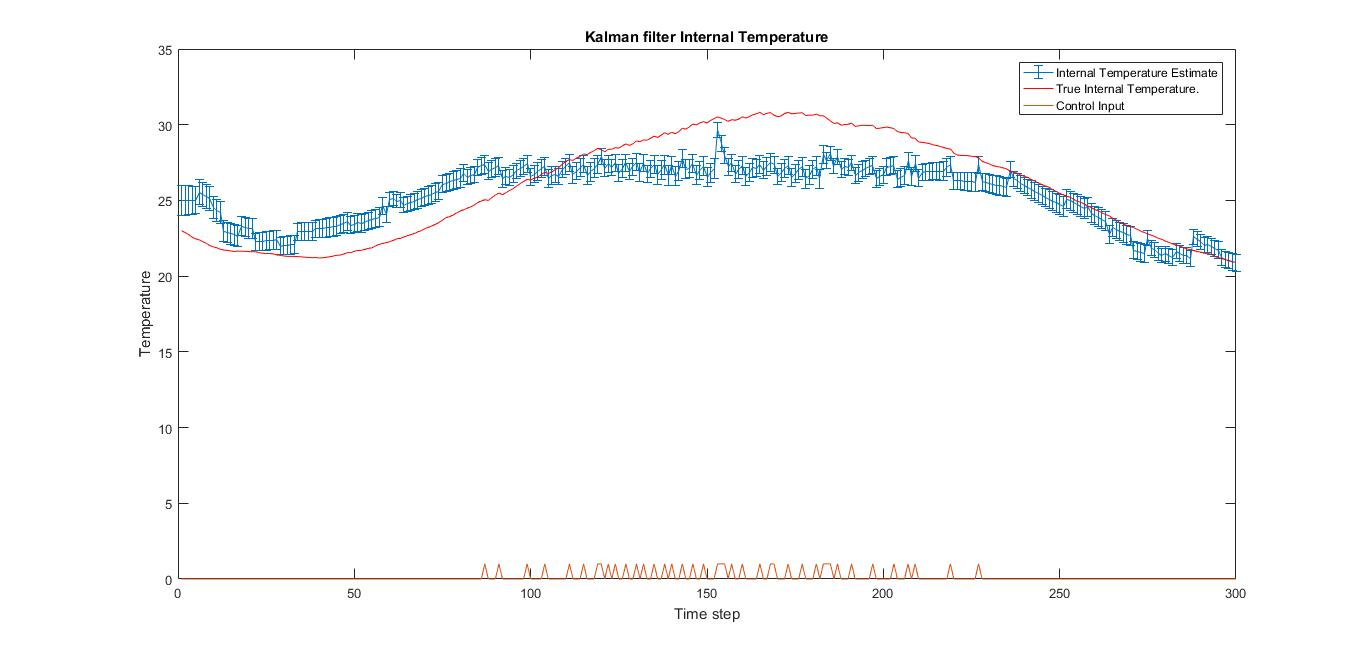
\includegraphics[scale=0.45]{q3_a}
   \caption{Kalman Filter for Tempreture control}\label{fig:q3}
\end{figure}
\clearpage
\newpage
\subsection*{(b)}
\begin{figure}[h]
  \hspace*{-5cm}
   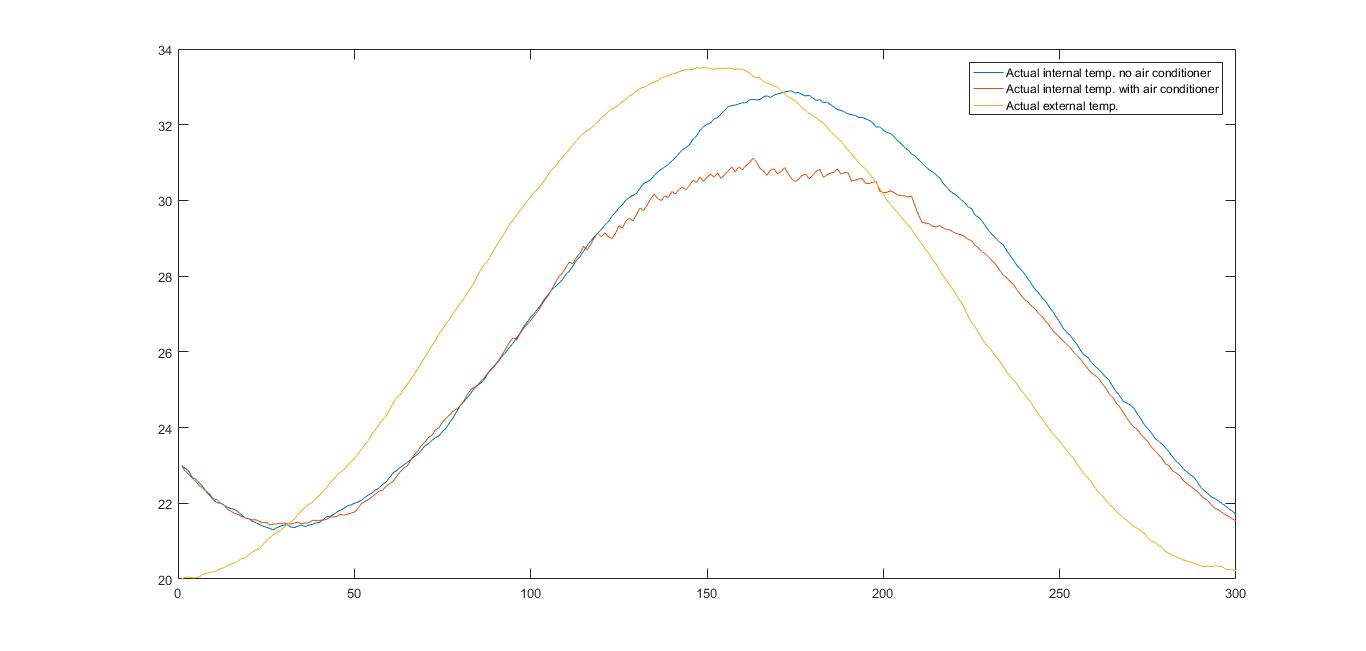
\includegraphics[scale=0.45]{q3_b}
   \caption{Kalman Filter for Tempreture control}\label{fig:q3}
\end{figure}
\quad \\
The internal temperature swings with in an acceptable range (doesn't go beyond 29-30 degrees) where as internal temperature without the air conditioner could go upto 33 degrees .

\clearpage
\newpage
\begin{appendix}
\section*{Code Appendix}
\lstinputlisting[language=Octave]{create_graph.m} -
\lstinputlisting[language=Octave]{hm9.m} 
\lstinputlisting[language=Octave]{newKalman.m} 
\lstinputlisting[language=Octave]{get_measurment.m} 

\end{appendix}•
\end{document}